\documentclass[aspectratio=169]{beamer}

% ---- Visual style, aligned with the provided template ----
\usepackage{xcolor}
\definecolor{HermesOrange}{HTML}{F37021}
\definecolor{SoftBlue}{HTML}{EAF3FF}
\definecolor{SoftGreen}{HTML}{EAF7EF}
\definecolor{SoftRed}{HTML}{FFF0EC}
\definecolor{SoftYellow}{HTML}{FFF7D8}
\definecolor{SoftPurple}{HTML}{F0ECFF}
\definecolor{SoftGray}{HTML}{F6F6F6}
\usetheme{Madrid}
\usecolortheme{seahorse}
\setbeamercolor{structure}{fg=HermesOrange}
\setbeamercolor{frametitle}{bg=HermesOrange!10, fg=black!90}
\setbeamercolor{title}{fg=HermesOrange}
\setbeamercolor{block title}{bg=HermesOrange!15, fg=black!90}
\setbeamercolor{block body}{bg=black!2, fg=black!92}
\setbeamercolor{item}{fg=HermesOrange}
\setbeamertemplate{navigation symbols}{}
\setbeamertemplate{itemize item}{\textcolor{HermesOrange}{$\blacktriangleright$}}
\setbeamertemplate{itemize subitem}{\textcolor{HermesOrange}{$\triangleright$}}
\setbeamertemplate{enumerate item}{\textcolor{HermesOrange}{\insertenumlabel.}}

\usepackage{amsmath,amssymb}
\usepackage{array}
\usepackage{booktabs}
\usepackage{tikz}
\usetikzlibrary{arrows.meta,positioning,calc,fit}
\newcommand{\paper}[1]{\textcolor{HermesOrange!90!black}{\textbf{#1}}}
\newcommand{\stlG}{\mathbf{G}}
\newcommand{\stlF}{\mathbf{F}}
\newcolumntype{L}[1]{>{\raggedright\arraybackslash}p{#1}}

\title[NL, STL, and Safe RL]{NL, STL, and Safe RL}
\author{Yuhang Zhang}
\institute{EECS, Washington State University}
\date{\today}

\begin{document}

% ===== 1 =====
\begin{frame}{From Natural Language to Safe RL: Three Complementary Pieces}
\begin{center}
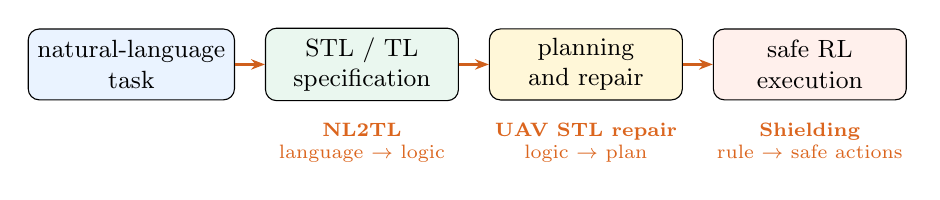
\begin{tikzpicture}[
  box/.style={draw,rounded corners,align=center,font=\small,minimum width=2.45cm,minimum height=0.9cm},
  note/.style={align=center,font=\scriptsize,text=HermesOrange!90!black},
  arr/.style={-{Stealth[length=5pt]},thick,HermesOrange!85!black}
]
  \node[box,fill=SoftBlue] (nl) {natural-language\\task};
  \node[box,fill=SoftGreen,right=0.38cm of nl] (stl) {STL / TL\\specification};
  \node[box,fill=SoftYellow,right=0.38cm of stl] (plan) {planning\\and repair};
  \node[box,fill=SoftRed,right=0.38cm of plan] (safe) {safe RL\\execution};
  \draw[arr] (nl)--(stl);
  \draw[arr] (stl)--(plan);
  \draw[arr] (plan)--(safe);
  \node[note,below=0.16cm of stl] {\paper{NL2TL}\\language \(\to\) logic};
  \node[note,below=0.16cm of plan] {\paper{UAV STL repair}\\logic \(\to\) plan};
  \node[note,below=0.16cm of safe] {\paper{Shielding}\\rule \(\to\) safe actions};
\end{tikzpicture}
\end{center}

\vspace{0.45em}
\begin{block}{Main message}
\small
The papers form a natural pipeline, but each starts and stops at a different boundary. Together they motivate a focused gap: \textbf{natural-language safety requirements should become grounded STL constraints that are usable and measurable inside RL}.
\end{block}
\end{frame}

% ===== 2 =====
\begin{frame}{Paper 1: NL2TL (EMNLP 2023)}
\begin{columns}[T]
\column{0.49\textwidth}
\begin{block}{Problem}
\footnotesize
Translate natural-language instructions into temporal logic across domains, despite limited manually labeled NL--TL pairs.
\end{block}

\begin{block}{Method}
\footnotesize
\begin{itemize}
  \item Replace concrete objects/actions with placeholders: \texttt{prop\_1}, \texttt{prop\_2}, \ldots
  \item Fine-tune T5 on lifted NL--STL pairs to learn temporal operators and formula structure.
  \item Use GPT-3 to synthesize data and detect atomic propositions in full natural language.
\end{itemize}
\end{block}

\column{0.47\textwidth}
\begin{block}{Example}
\scriptsize
\[
\begin{array}{c}
\text{``eventually visit A''}\\[-0.15em]
\text{``and always avoid B''}\\[0.15em]
\Downarrow\\[0.15em]
\stlF\,\texttt{prop\_1}\wedge \stlG\,\neg\texttt{prop\_2}.
\end{array}
\]
\end{block}

\begin{block}{Takeaway}
\footnotesize
T5-large reaches about \(97.5\%\) exact match on lifted data; full NL-to-STL with GPT-3 AP detection is around \(95\%\)--\(97\%\). The paper is a strong \textbf{language-to-specification front end}, not a safety execution method.
\end{block}
\end{columns}
\end{frame}

% ===== 3 =====
\begin{frame}{Paper 2: UAV NL-to-STL with MILP Repair (2026)}
\begin{center}
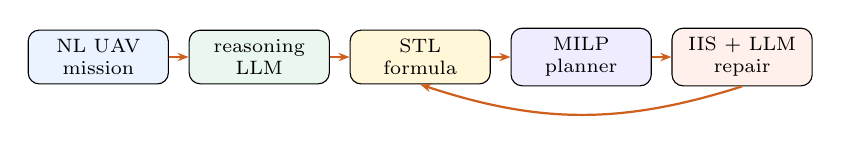
\begin{tikzpicture}[
  box/.style={draw,rounded corners,align=center,font=\scriptsize,minimum width=1.78cm,minimum height=0.68cm},
  arr/.style={-{Stealth[length=4pt]},thick,HermesOrange!85!black}
]
  \node[box,fill=SoftBlue] (nl) {NL UAV\\mission};
  \node[box,fill=SoftGreen,right=0.25cm of nl] (llm) {reasoning\\LLM};
  \node[box,fill=SoftYellow,right=0.25cm of llm] (stl) {STL\\formula};
  \node[box,fill=SoftPurple,right=0.25cm of stl] (milp) {MILP\\planner};
  \node[box,fill=SoftRed,right=0.25cm of milp] (repair) {IIS + LLM\\repair};
  \draw[arr] (nl)--(llm);
  \draw[arr] (llm)--(stl);
  \draw[arr] (stl)--(milp);
  \draw[arr] (milp)--(repair);
  \draw[arr] (repair.south) to[bend left=18] (stl.south);
\end{tikzpicture}
\end{center}

\vspace{0.2em}
\begin{columns}[T]
\column{0.52\textwidth}
\begin{block}{Core idea}
\footnotesize
The paper connects translation to execution: STL satisfaction and UAV dynamics are encoded into a mixed-integer linear program. If no trajectory exists, IIS diagnosis maps conflicts back to STL subformulas, and an LLM chooses a repair direction.
\end{block}

\column{0.44\textwidth}
\begin{block}{Safety-aware repair}
\footnotesize
\[
\stlG_{[0,T]}\neg R_o \wedge \stlF_{[0,20]}R_g
\leadsto
\stlG_{[0,T]}\neg R_o \wedge \stlF_{[0,30]}R_g .
\]
The obstacle-avoidance rule remains hard; only the deadline is relaxed.
\end{block}
\end{columns}
\end{frame}

% ===== 4 =====
\begin{frame}{Paper 3: Safe RL via Shielding (2017)}
\begin{columns}[T]
\column{0.48\textwidth}
\begin{block}{Problem}
\footnotesize
RL may maximize reward while violating safety during training or deployment. Reward penalties alone do not provide formal guarantees.
\end{block}

\begin{block}{Method}
\footnotesize
Given a temporal-logic safety rule \(\varphi_s\) and a conservative finite-state abstraction, synthesize a shield that filters or corrects unsafe actions before they can force a future violation.
\end{block}

\column{0.48\textwidth}
\begin{center}
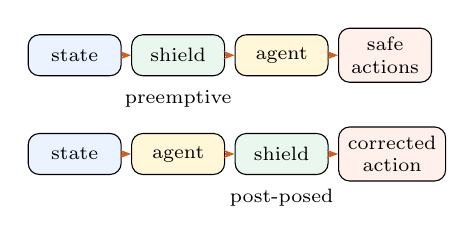
\begin{tikzpicture}[
  box/.style={draw,rounded corners,align=center,font=\scriptsize,minimum width=1.18cm,minimum height=0.52cm},
  arr/.style={-{Stealth[length=4pt]},thick,HermesOrange!85!black}
]
  \node[box,fill=SoftBlue] (env1) {state};
  \node[box,fill=SoftGreen,right=0.12cm of env1] (sh1) {shield};
  \node[box,fill=SoftYellow,right=0.12cm of sh1] (ag1) {agent};
  \node[box,fill=SoftRed,right=0.12cm of ag1] (act1) {safe\\actions};
  \draw[arr] (env1)--(sh1);
  \draw[arr] (sh1)--(ag1);
  \draw[arr] (ag1)--(act1);
  \node[font=\scriptsize,below=0.05cm of sh1] {preemptive};

  \node[box,fill=SoftBlue,below=0.72cm of env1] (env2) {state};
  \node[box,fill=SoftYellow,right=0.12cm of env2] (ag2) {agent};
  \node[box,fill=SoftGreen,right=0.12cm of ag2] (sh2) {shield};
  \node[box,fill=SoftRed,right=0.12cm of sh2] (act2) {corrected\\action};
  \draw[arr] (env2)--(ag2);
  \draw[arr] (ag2)--(sh2);
  \draw[arr] (sh2)--(act2);
  \node[font=\scriptsize,below=0.05cm of sh2] {post-posed};
\end{tikzpicture}
\end{center}

\begin{block}{Takeaway}
\footnotesize
Shielding is the strongest RL safety-execution piece, but it assumes the formal safety rule and environment abstraction are already available.
\end{block}
\end{columns}
\end{frame}

% ===== 5 =====
\begin{frame}{What Each Paper Gives, and What Is Still Missing}
\footnotesize
\renewcommand{\arraystretch}{1.18}
\setlength{\tabcolsep}{3pt}
\begin{tabular}{L{0.19\textwidth} L{0.24\textwidth} L{0.25\textwidth} L{0.23\textwidth}}
\toprule
\textbf{Paper} & \textbf{Solves} & \textbf{Strength} & \textbf{Missing for us} \\
\midrule
\paper{NL2TL} & Natural language \(\to\) STL/TL formula & Strong cross-domain translation via lifted APs and T5 & No trajectory-level safety or RL execution \\
\paper{UAV STL repair} & STL formula \(\to\) feasible UAV trajectory or repaired task & Formal MILP feasibility and safety-preserving repair & Model-based planning, not policy learning \\
\paper{Shielding} & Given safety rule \(\to\) safe RL actions & Runtime enforcement during learning and execution & Assumes expert-written rule and abstraction \\
\bottomrule
\end{tabular}

\vspace{0.8em}
\begin{block}{Synthesis}
\footnotesize
The missing piece is not another isolated translator, planner, or shield. It is the interface that turns \textbf{natural-language safety requirements} into \textbf{grounded STL constraints} whose effect can be evaluated on RL trajectories.
\end{block}
\end{frame}

% ===== 6 =====
\begin{frame}{Our Focused Problem}
\begin{block}{Problem definition}
\footnotesize
Given an RL environment \(M\) and a language task \(L=(L_{\mathrm{goal}},L_{\mathrm{safe}})\), translate and ground \(L_{\mathrm{safe}}\) into an STL safety constraint \(\varphi_{\mathrm{safe}}\), then train or evaluate policies under trajectory-level safety:
{\scriptsize
\[
\max_{\pi}\ \mathbb{E}_{\pi}\!\left[\sum_{t=0}^{H}\gamma^t r_t\right]
\quad
\text{s.t.}\quad
\Pr_{\tau\sim\pi}\!\left[\tau \models \varphi_{\mathrm{safe}}\right]\ge 1-\delta .
\]
}
\end{block}

\begin{columns}[T]
\column{0.49\textwidth}
\begin{block}{First-stage scope}
\footnotesize
\begin{itemize}
  \item Focus on the safety part of language tasks.
  \item Ground vague requirements into predicates and time windows.
  \item Evaluate violation rate, STL robustness, task success, and intervention count.
\end{itemize}
\end{block}

\column{0.47\textwidth}
\begin{block}{Why it follows naturally}
\footnotesize
\begin{itemize}
  \item NL2TL gives translation, but not enforcement.
  \item UAV repair gives feasibility, but not RL learning.
  \item Shielding gives RL enforcement, but not language grounding.
\end{itemize}
\end{block}
\end{columns}
\end{frame}

\end{document}
